\begin{figure}[h!]
	\centering
	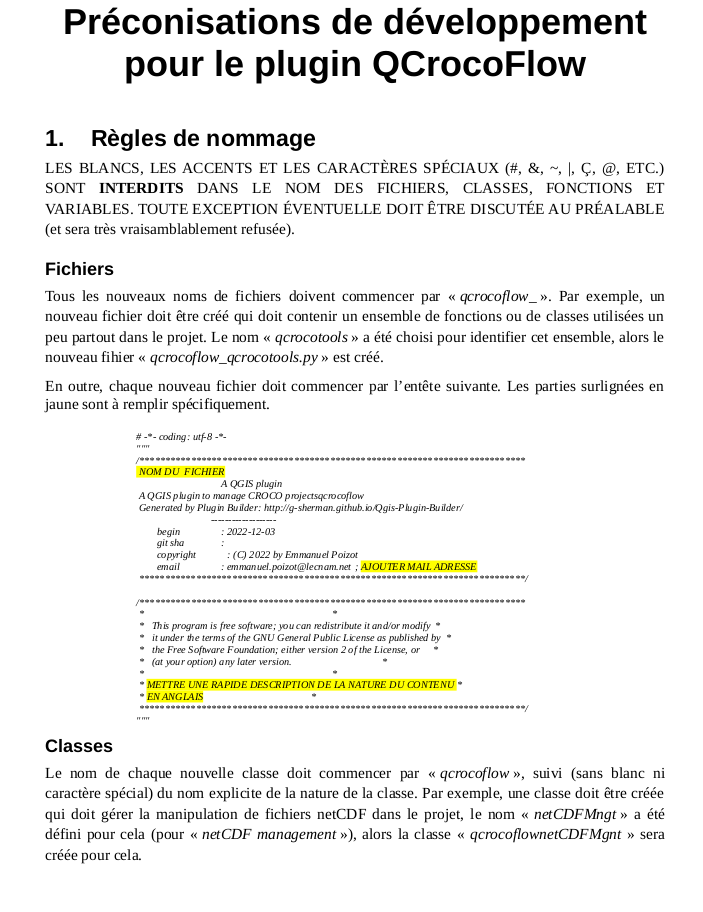
\includegraphics[width=0.9\textwidth]{./IMAGES/Annexe/annexe1.png}
\end{figure}
%---------------------------------------------------------------------
\newpage
\begin{figure}[h!]
	\centering
	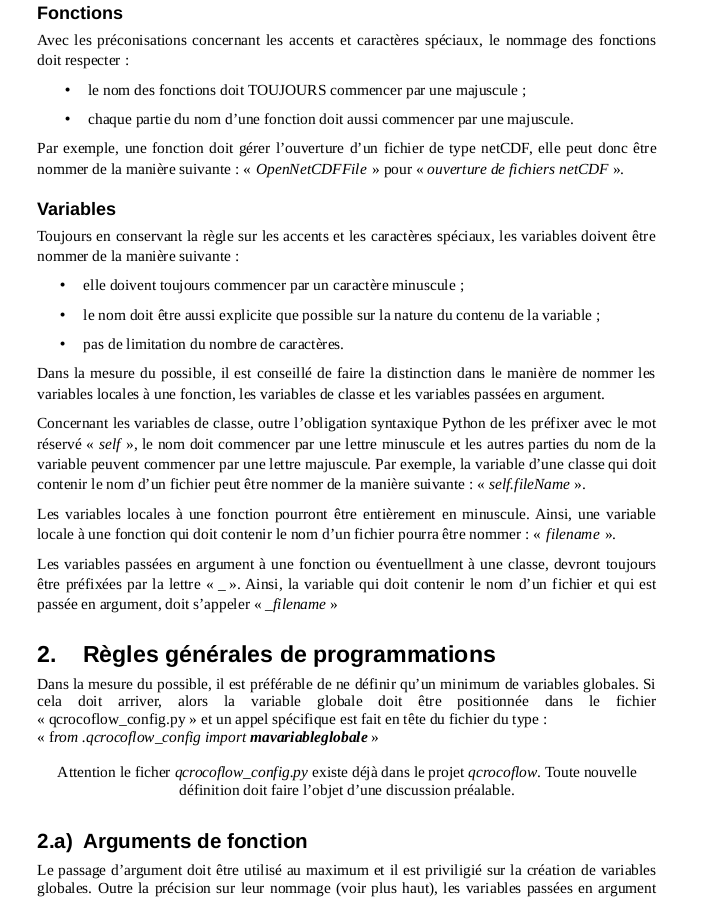
\includegraphics[width=0.9\textwidth]{./IMAGES/Annexe/annexe2.png}
\end{figure}
%---------------------------------------------------------------------
\newpage
\begin{figure}[h!]
	\centering
	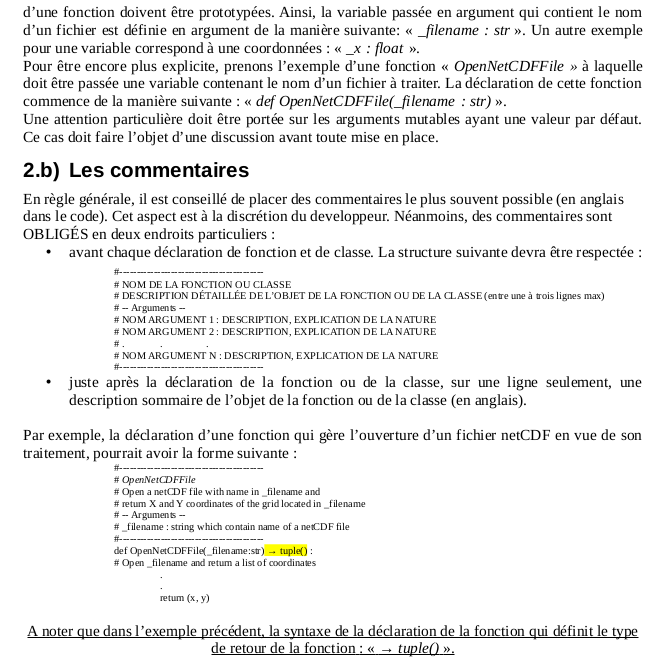
\includegraphics[width=1\textwidth]{./IMAGES/Annexe/annexe3.png}
\end{figure}

\subsection*{Code Source}
Le code source associé aux scripts est disponible en libre accès sur GitHub. En raison de la longueur et de la complexité des scripts, il est préférable de les consulter directement sur le dépôt GitHub plutôt que de les inclure dans cette annexe.

Les scripts font partie du projet \textit{qcrocoflow} et sont situés dans le dossier `preprocess`. Chaque fonction est soigneusement commentée et expliquée pour faciliter la compréhension et l'utilisation.

Vous pouvez accéder au code source en suivant ce lien : \href{https://github.com/epzt/qcrocoflow}{https://github.com/epzt/qcrocoflow}.
